\chapter{Implementasi dan Pengujian}
\label{chap:implementasidanpengujian}
Bab ini berisi Implementasi Perangkat Lunak dan Pengujian Perangkat Lunak. Bagian implementasi terdiri dari penjelasan lingkungan pengembangan perangkat lunak dan hasil implementasi. Bagian pengujian terdiri dari hasil pengujian fungsional dan eksperimental terhadap perangkat lunak yang telah dibangun.

\section{Implementasi}
\label{sec:implementasi} 

\subsection{Lingkungan Implementasi}
Implementasi perangkat lunak ini dilakukan pada komputer penulis dengan spesifikasi berikut:
\begin{enumerate}
	\item \textit{Processor}: Intel Core i5 9400F
	\item \textit{Random Access Memory} (RAM): 16 GB DDR4
	\item Sistem Operasi: Windows 10
	\item Versi Python : Python 3.8.5
\end{enumerate}

\subsection{Hasil Implementasi}
Hasil implementasi berupa sebuah perangkat lunak perekaman kehadiran daring otomatis dengan bahasa pemrograman python. Sebelum menjalankan perangkat lunak untuk perekaman kehadiran daring otomatis, terdapat \textit{file} .ini yang merupakan sebuah masukkan untuk perangkat lunak. \textit{File} .ini dibahas pada Subbab \ref{sec:inputConfig}. Contoh \textit{file} .ini dapat dilihat pada \ref{kode:5:kodemasukan}.
\begin{lstlisting}[caption=Contoh \textit{file} .ini untuk Masukan Perangkat Lunak Perekaman Kehadiran Daring Otomatis, label=kode:5:kodemasukan]
	[database_config]
	1 = open https://studentportal.unpar.ac.id
	2 = click #login-button
	3 = sendkeys #username 2017730035@student.unpar.ac.id 
	4 = click #next_login
	5 = sendkeys #password 12345
	6 = click #appPass>div.login__form>button
	7 = or a[href='https://studentportal.unpar.ac.id/jadwal'] .swal-button.swal-button--confirm.swal-button--danger
	8 = click a[onclick="absenPerkuliahan(this)"]
	9 = click .swal-button.swal-button--confirm.swal-button--danger9
	10 = quit
\end{lstlisting}

Perekaman kehadiran daring otomatis dapat dilakukan dengan menjalankan perangkat lunak. Pengguna perlu membuka \textit{Command Prompt} pada komputer maupun laptop dengan \textit{directory} file automatedTesting.py berada dan menuliskan perintah ``python automatedTesting.py'' atau ``py automatedTesting.py'' pada \textit{Command Prompt}, seperti pada tampilan Gambar \ref{fig:cmd}
\begin{figure}[H]
	\centering
	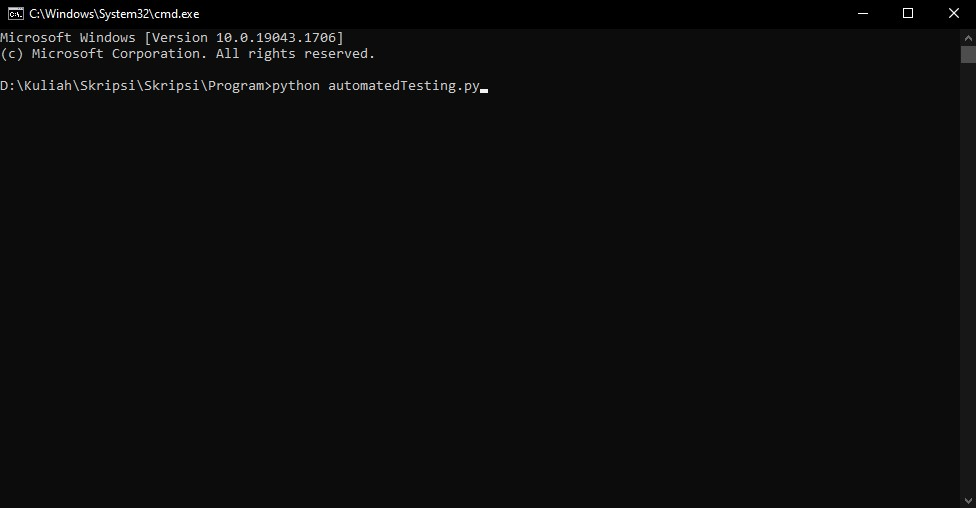
\includegraphics[scale=0.5]{Gambar/cmd.jpg}
	\caption{Tampilan \textit{Command Prompt} dengan \textit{Directory File}} 
	\label{fig:cmd}
\end{figure}

Setelah pengguna menekan ``Enter'' pada \textit{Command Prompt} maka perangkat lunak akan melakukan perekaman kehadiran daring secara otomatis, bagi mahasiswa maka perangkat lunak akan melakukan perekaman kehadiran daring pada Portal Akademik Mahasiswa secara otomatis, dimana perangkat lunak akan menjalankan secara otomatis tahap-tahap perekaman kehadiran daring secara manual yang biasa dilakukan mahasiswa seperti yang dibahas pada Subbab \ref{sec:alur}, sedangkan bagi dosen maka perangkat lunak akan melakukan perekaman kehadiran daring pada AKUHADIR seperti yang dibahas pada Subbab \ref{sec:akuhadir}. Setelah berhasil melakukan perekaman kehadiran daring maka akan muncul pemberitahuan pada \textit{Command Prompt} dengan tulisan ``Information: Absensi Berhasil!'' bahwa perekaman berhasil dilakukan. Pemberitahuan absensi gagal pada \textit{Command Prompt} akan ada tulisan ``Warning! Absensi Gagal, Elemen tidak ditemukan: (\textit{diisi dengan sesuai elemen yang tidak ditemukan})''. Absensi gagal terjadi karena tidak ada jadwal kuliah lagi bagi mahasiswa, atau sudah melakukan absensi sehingga tidak ada yang bisa lagi untuk melakukan perekaman kehadiran.

\section{Pengujian}
\label{sec:pengujian} 

\subsection{Pengujian Fungsional Mahasiswa}
Pengujian fungsional dilakukan untuk mengetahui kesesuaian reaksi perangkat lunak dengan reaksi yang diharapkan berdasarkan aksi pengguna terhadap perangkat lunak. Tabel \ref{tab:fungsiMahasiswa} merupakan tabel hasil pengujian perangkat lunak pada komputer penulis dengan spesifikasi berikut:
\begin{enumerate}
	\item \textit{Processor}: Intel Core i5 9400F
	\item \textit{Random Access Memory} (RAM): 16 GB DDR4
	\item Sistem Operasi: Windows 10
	\item Versi Python : Python 3.8.5
\end{enumerate}
Mahasiswa melakukan perekaman kehadiran otomatis di Portal Akademik Mahasiswa. Mahasiswa perlu penyesuaian \textit{file} \texttt{database.ini} seperti dilihat pada kode \ref{kode:5:databasemahasiswa}.
\\
\begin{lstlisting}[caption=\textit{File} \texttt{database.ini} Portal Akademik Mahasiswa (\textit{password} disembunyikan), label=kode:5:databasemahasiswa]
	[database_config]
	1 = open https://studentportal.unpar.ac.id
	2 = click #login-button
	3 = sendkeys #username 2017730035@student.unpar.ac.id 
	4 = click #next_login
	5 = sendkeys #password 12345
	6 = click #appPass>div.login__form>button
	7 = or a[href='https://studentportal.unpar.ac.id/jadwal'] .swal-button.swal-button--confirm.swal-button--danger
	8 = click a[onclick="absenPerkuliahan(this)"]
	9 = click .swal-button.swal-button--confirm.swal-button--danger
	10 = quit
\end{lstlisting}


Setelah menjalankan program, didapatkan bahwa program dapat berjalan dan berfungsi dengan baik untuk dapat melakukan perekaman kehadiran daring otomatis pada situs Portal Akademik Mahasiswa. Kesimpulan dari pengujian fungsional mahasiswa pada program dinyatakan berhasil, dan selengkapnya dapat dilihat pada tabel \ref{tab:fungsiMahasiswa}.

\begin{table}[H]			
	\caption{Tabel Pengujian Fungsional}
	\centering
	\begin{tabular}{|p{0.5cm} |p{4cm} |p{5.5cm}| p{3cm}|} \hline
		No. & Aksi Pengguna & Reaksi yang diharapkan & Reaksi Perangkat Lunak\\ \hline     
		1. 	& Mahasiswa menjalankan perangkat lunak & Browser Google Chrome terbuka & Sesuai\\ \hline 
	 		& &  Browser menuju situs Portal Akademik Mahasiswa & Sesuai\\ \hline 
			& &  Browser menuju halaman web untuk perekaman kehadiran daring & Sesuai\\ \hline 
			& &  Melakukan perekaman kehadiran daring secara otomatis & Sesuai\\ \hline
	\end{tabular}
	\label{tab:fungsiMahasiswa}
\end{table}

\subsection{Pengujian Fungsional Dosen}

\textit{Subbab ini ditulis berdasarkan hasil wawancara terhadap dosen pembimbing ketika mencoba program perekaman kehadiran daring otomatis.}

Program yang sudah dibuat diujikan juga di komputer dosen pembimbing, untuk melakukan rekam kehadiran pada portal AKUHADIR (subbab \ref{sec:akuhadir}). Berikut adalah spesifikasi komputer dosen pembimbing yang digunakan untuk menguji:

\begin{enumerate}
	\item \textit{Processor}: Apple M1
	\item \textit{Random Access Memory} (RAM): 8 GB
	\item Sistem Operasi: macOS Monterey
	\item Versi Python : Python 3.9.10
\end{enumerate}

Dosen pembimbing melakukan perekaman kehadiran otomatis di AKUHADIR. Dosen pembimbing perlu penyesuaian \textit{file} \texttt{database.ini} seperti dilihat pada kode \ref{kode:5:databasedosen}.

\begin{lstlisting}[caption=\textit{File} \texttt{database.ini} AKUHADIR (\textit{password} disembunyikan), label=kode:5:databasedosen]
[database_config]
1 = open https://akuhadir.unpar.ac.id
2 = sendkeys #username pascal@unpar.ac.id
3 = click #next_login
4 = sendkeys #password xxx
5 = click button[name=submit]
6 = click a[href='https://akuhadir.unpar.ac.id/absensi?tab=tab2']
7 = click a[onclick='checkin_home()']
8 = quit
\end{lstlisting}


Setelah dosen pembimbing menjalankan program, didapatkan bahwa program dapat berjalan dan berfungsi dengan baik untuk dapat melakukan perekaman kehadiran daring otomatis pada situs AKUHADIR. Kesimpulan dari pengujian fungsional program pada komputer dosen pembimbing dinyatakan berhasil, dan selengkapnya dapat dilihat pada tabel \ref{tab:fungsidosen}.

\begin{table}[H]			
	\caption{Tabel Pengujian Fungsional}
	\centering
	\begin{tabular}{|p{0.5cm} |p{4cm} |p{5.5cm}| p{3cm}|} \hline
		No. & Aksi Pengguna & Reaksi yang diharapkan & Reaksi Perangkat Lunak\\ \hline     
		1. & Dosen menjalankan perangkat lunak & Browser Google Chrome terbuka & Sesuai\\ \hline 
		 	& &  Browser menuju situs AKUHADIR & Sesuai\\ \hline
		 	& &  Browser menuju halaman web untuk perekaman kehadiran & Sesuai\\ \hline
		 	& &  Melakukan perekaman kehadiran daring secara otomatis & Sesuai\\ \hline
	\end{tabular}
	\label{tab:fungsidosen}
\end{table}

\subsection{Pengujian Eksperimental}
Pengujian eksperimental dilakukan terhadap beberapa mahasiswa dan dosen Universitas Katolik Parahyangan jurusan Teknik Informatika yang sudah memiliki Google Chrome dan Python3. Metode pengujian dilakukan dengan cara menyebarkan perangkat lunak yang dapat diunduh melalui Google Drive. Setelah menjalankan perangkat lunak tersebut, mahasiswa dan dosen diminta untuk mengisi Google Form untuk mengetahui kelancaran perangkat lunak ketika dijalankan dan mengetahui lama waktu yang dibutuhkan hingga program berhasil melakukan perekaman kehadiran. 

\subsubsection{Hasil Survei Mahasiswa}
Dari 7 responden yang telah mengisi survei, memberi respons bahwa perangkat lunak berjalan dengan baik dan dapat melakukan perekaman kehadiran daring secara otomatis. Pertanyaan yang diajukan kepada responen dan rangkuman jawaban hasil survei sebagai berikut:
\begin{enumerate}
	\item \textbf{Apakah perangkat lunak berjalan dengan baik (tidak ada crash atau error) dan dapat melakukan perekaman kehadiran daring secara otomatis?}
	
	Berdasarkan jawaban dari semua responden menyatakan setuju bahwa program tidak mengalami \textit{error} atau \textit{crash}.
	\item \textbf{Setelah menjalankan perangkat lunak perekaman kehadiran daring otomatis. Berapa lama(detik) waktu yang dibutuhkan untuk melakukan perekaman kehadiran daring menggunakan program perekaman kehadiran daring otomatis?}
	
	Histogram ini dikelompokan berdasarkan rentang waktu per 20 detik. Histogram menunjukan bahwa sebanyak 6 mahasiswa memiliki rentang waktu 0 sampai 20 detik dan sebanyak 1 mahasiswa memiliki rentang waktu 21 sampai 40 detik. 
	\begin{figure}[H]
		\centering
		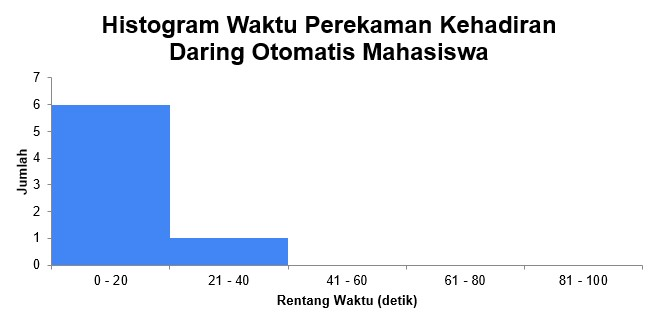
\includegraphics[scale=0.75]{Gambar/HistogramDaringOtomatisMahasiswa.jpg}
		\caption{Histogram Waktu Perekaman Kehadiran Daring Otomatis Mahasiswa}
		\label{fig:olMahasiswa}
	\end{figure}
	Hasil survei perekaman kehadiran daring otomatis untuk setiap mahasiswa secara jelas dapat dilihat pada tabel \ref{tab:otomatis} menunjukan waktu yang didapatkan dari 7 responden dalam menjalankan perangkat lunak untuk melakukan perekaman kehadiran daring otomatis. Hasil tabel tersebut menunjukan bahwa dalam melakukan perekaman kehadiran daring otomatis memiliki rata-rata waktu adalah 16,71 detik.
	\begin{table}[ht]			
		\caption{Tabel Perekaman Kehadiran Daring Otomatis Mahasiswa}
		\centering
		\begin{tabular}{|p{3.5cm} |p{7cm}|}
			\hline
			Jumlah Responden &  Waktu Perekaman Kehadiran Otomatis \\ \hline     
			1 orang &  11 detik\\ \hline 
			1 orang &  14 detik\\ \hline 
			1 orang &  15 detik\\ \hline 
			2 orang &  18 detik\\ \hline 
			1 orang &  19 detik\\ \hline 
			1 orang &  22 detik\\ \hline 
		\end{tabular}
		\label{tab:otomatis}
	\end{table}
	\item \textbf{Apakah setuju dengan perangkat lunak perekaman kehadiran daring otomatis ini, membuat waktu interaksi dengan situs web/browser untuk melakukan absensi menjadi lebih singkat?}
	
	Berdasarkan jawaban dari semua responden menyatakan setuju bahwa perangkat lunak untuk melakukan perekaman kehadiran daring secara otomatis dapat membuat waktu interaksi dengan situs web atau browser menjadi lebih singkat.
\end{enumerate}

	
\subsubsection{Hasil Survei Dosen}
Hasil survei kepada dosen hanya mendapat 2 respon dosen. Pertanyaan yang diajukan kepada responen dan rangkuman jawaban hasil survei sebagai berikut:
\begin{enumerate}
	\item \textbf{Apakah perangkat lunak berjalan dengan baik (tidak ada crash atau error) dan dapat melakukan perekaman kehadiran daring secara otomatis?}
	
	Berdasarkan jawaban dari semua responden menyatakan setuju bahwa program tidak mengalami \textit{error} atau \textit{crash}.
	\newpage
	\item \textbf{Setelah menjalankan perangkat lunak perekaman kehadiran daring otomatis. Berapa lama(detik) waktu yang dibutuhkan untuk melakukan perekaman kehadiran daring menggunakan program perekaman kehadiran daring otomatis?}
	
	Dua dosen yang menjadi responden menyatakan waktu yang dibutuhkan untuk melakukan perekaman kehadiran daring secara otomatis adalah 2 detik dan 15 detik. Rata-rata perekaman kehadiran daring otomatis yang dilakukan oleh dua dosen tersebut adalah 8,5 detik. 

	\item \textbf{Apakah setuju dengan perangkat lunak perekaman kehadiran daring otomatis ini, membuat waktu interaksi dengan situs web/browser untuk melakukan absensi menjadi lebih singkat?}
	
	Berdasarkan jawaban dari semua responden menyatakan setuju bahwa perangkat lunak untuk melakukan perekaman kehadiran daring secara otomatis dapat membuat waktu interaksi dengan situs web atau browser menjadi lebih singkat.
\end{enumerate}


\subsubsection{Perbandingan Hasil Pengujian}
Bagian ini akan membandingkan waktu yang didapatkan perekaman kehadiran daring secara otomatis menggunakan program dengan waktu perekaman kehadiran daring dan luring bagi mahasiswa maupun dosen yang didapatkan dari survei pada subbab \ref{sec:survei}. Tabel \ref{tab:banding} merupakan tabel hasil perbandingan rata-rata waktu untuk melakukan perekaman kehadiran.
\begin{table}[H]			
 	\caption{Tabel Perekaman kehadiran}
 	\centering
 	\begin{tabular}{|p{2cm} |p{4cm} |p{4cm}| p{4cm}|} \hline
 		Pengguna & Rata-rata waktu dengan program & Rata-rata waktu luring & Rata-rata waktu daring\\ \hline     
 		Mahasiswa & 16,71 detik (7 respon)& 7,95 detik (21 respon)& 63 detik (21 respon)\\ \hline 
 		Dosen & 8,5 detik (2 respon)&  24,33 detik (6 respon)& 31,83 detik (6 respon)\\ \hline 
 	\end{tabular}
 	\label{tab:banding} 
\end{table}
Dari hasil perbandingan pada tabel \ref{tab:banding} secara angka dapat dilihat bahwa untuk mahasiswa waktu perekaman kehadiran dengan program masih lebih lama sedikit dengan waktu perekaman luring tetapi lebih cepat dibanding waktu perekaman daring dan untuk dosen perekaman kehadiran dengan perangkat lunak lebih cepat dibandingkan waktu perekaman daring maupun luring.